\documentclass[12pt,twocolumn,tighten]{aastex62}
%\pdfoutput=1 %for arXiv submission
\usepackage{amsmath,amstext,amssymb}
\usepackage[T1]{fontenc}
\usepackage{apjfonts}
\usepackage[figure,figure*]{hypcap}
\usepackage{graphics,graphicx}
\usepackage{hyperref}
\usepackage{comment}

\renewcommand*{\sectionautorefname}{Section} %for \autoref
\renewcommand*{\subsectionautorefname}{Section} %for \autoref

%% Reintroduced the \received and \accepted commands from AASTeX v5.2.
%% Add "Submitted to " argument.
\received{\today}
\revised{---}
\accepted{---}
\submitjournal{AAS journals.}

\shortauthors{Bouma et al.}
\shorttitle{CDIPS I: Method \& Sector 6}

%%%%%%%%%%%%%%%%%%%%%%%%%%%%%%%%%%%%%%%%%%
% BEGIN CUSTOM SHORT-CUT COMMANDS

% BEGIN CLUSTER TABLE
%FIXME: write code that will write these values
\newcommand{\cgXVIIInstartot}{}
\newcommand{\cgXVIIInstarcdipsI}{}
\newcommand{\gaiaXVIIInstartot}{}
\newcommand{\gaiaXVIIInstarcdipsI}{}

\newcommand{\kXIIInstartot}{}
\newcommand{\kXIIInstarcdipsI}{}
\newcommand{\dXIVnstartot}{}
\newcommand{\dXIVnstarcdipsI}{}
\newcommand{\bellXVIInstartot}{}
\newcommand{\bellXVIInstarcdipsI}{}
\newcommand{\banyanXIIInstartot}{}
\newcommand{\banyanXIIInstarcdipsI}{}
\newcommand{\banyanXIInstartot}{}
\newcommand{\banyanXIInstarcdipsI}{}
\newcommand{\banyanXInstartot}{}
\newcommand{\banyanXInstarcdipsI}{}
\newcommand{\krausXIVnstartot}{}
\newcommand{\krausXIVnstarcdipsI}{}
\newcommand{\ohXVIInstartot}{}
\newcommand{\ohXVIInstarcdipsI}{}
\newcommand{\rizzutoXInstartot}{}
\newcommand{\rizzutoXInstarcdipsI}{}
\newcommand{\roserXInstartot}{}
\newcommand{\roserXInstarcdipsI}{}

\newcommand{\cgXVIIInclustertot}{}
\newcommand{\cgXVIIInclustercdipsI}{}
\newcommand{\gaiaXVIIInclustertot}{}
\newcommand{\gaiaXVIIInclustercdipsI}{}

\newcommand{\kXIIInclustertot}{}
\newcommand{\kXIIInclustercdipsI}{}
\newcommand{\dXIVnclustertot}{}
\newcommand{\dXIVnclustercdipsI}{}
\newcommand{\bellXVIInclustertot}{}
\newcommand{\bellXVIInclustercdipsI}{}
\newcommand{\banyanXIIInclustertot}{}
\newcommand{\banyanXIIInclustercdipsI}{}
\newcommand{\banyanXIInclustertot}{}
\newcommand{\banyanXIInclustercdipsI}{}
\newcommand{\banyanXInclustertot}{}
\newcommand{\banyanXInclustercdipsI}{}
\newcommand{\krausXIVnclustertot}{}
\newcommand{\krausXIVnclustercdipsI}{}
\newcommand{\ohXVIInclustertot}{}
\newcommand{\ohXVIInclustercdipsI}{}
\newcommand{\rizzutoXInclustertot}{}
\newcommand{\rizzutoXInclustercdipsI}{}
\newcommand{\roserXInclustertot}{}
\newcommand{\roserXInclustercdipsI}{}
% END CLUSTER TABLE

% END CUSTOM SHORT-CUT COMMANDS
%%%%%%%%%%%%%%%%%%%%%%%%%%%%%%%%%%%%%%%%%%

%%%%%

%\NewPageAfterKeywords

\begin{document}

\title{
  The Cluster Difference Imaging Photometric Survey (CDIPS).
  I. Method \& TESS Light Curves from Sector 6
}

\correspondingauthor{L. G. Bouma}
\email{luke@astro.princeton.edu}

\author[0000-0002-0514-5538]{L. G. Bouma}
\affiliation{ Department of Astrophysical Sciences, Princeton
University, 4 Ivy Lane, Princeton, NJ 08540, USA}
%
\author[0000-0002-0628-0088]{W. Bhatti}
\affiliation{ Department of Astrophysical Sciences, Princeton
    University, 4 Ivy Lane, Princeton, NJ 08540, USA}
%
\author[0000-0001-8732-6166]{J. D. Hartman}
\affiliation{ Department of Astrophysical Sciences, Princeton
University, 4 Ivy Lane, Princeton, NJ 08540, USA}
%
\author[0000-0001-7204-6727]{G. \'A. Bakos}
\affiliation{ Department of Astrophysical Sciences, Princeton
University, 4 Ivy Lane, Princeton, NJ 08540, USA}
%
\author[0000-0002-4265-047X]{J. N. Winn}
\affiliation{ Department of Astrophysical Sciences, Princeton
University, 4 Ivy Lane, Princeton, NJ 08540, USA}

\begin{abstract}
  Lorem ipsum.
\end{abstract}

\keywords{
  methods: data analysis ---
  techniques: photometric ---
  %TODO: could be individual, and enumerate each cluster as well.
  (Galaxy:) open clusters and associations: general ---
  planets and satellites: detection 
}


%%%%%%%%%%%%%%%%%%%%%%%%%%%%%%%%%%%%%%%%%%
\section{Introduction}
\label{sec:intro}

The exoplanet field is evolving.
At the beginning, Doppler spectroscopy by the Geneva and California groups
led to the first exoplanet detections (CITE: Mayor 95, Butler, Marcy).
Some of these planets transited (CITE: Henry, Charbonneau).
Despite the geometric rarity of transits, photometric monitoring can
be performed in parallel, while spectroscopy cannot.
This enabled thousands of planet detections with the Kepler spacecraft
(CITE: Borucki, Morton).
The abundance of planets from Kepler taught us about statistics
(CITE: Howard, Fressin, Petigura).
By nature of its design, Kepler left open two major avenues for
improvement: (i) brighter stars, (ii) rare weirdos.
TESS (CITE: Ricker), by nature of its small, wide-field cameras, and
nearly all-sky coverage, can capitalize on both.
TESS observes more stars than Kepler, for on average less time.
One class of rare weirdo to which TESS is sensitive is stars in
clusters.  For brevity, we use the term ``cluster'' to refer to open
clusters, moving groups, associations, and star-forming regions.
Each of the $\sim$1000 star clusters of the Milky Way is a gift to
astrophysics, providing a sample of stars that vary widely in mass
but all have approximately the same age and composition. 

Cluster stars have been monitored photometrically from the ground
(CITE: Joel thesis, Cambridge group).
A few clusters, NAME1 and NAME2, were observed by Kepler in its prime
mission (CITE: Meibom).
And a few more, most notably X,Y, and Z, were observed in K2's
ecliptic mission (CITE).

TESS holds the promise to deliver the most homogeneous and
comprehensive cluster photometric survey in history.  Based on the
cluster membership database of \citet{Kharchenko_et_al_2013} and the
TESS apparent magnitude calculator of \citet{Jaffe_Barclay_2017}, we
estimate that $10^5$ cluster members brighter than $T=16$ will be
observed in the northern ecliptic hemisphere's full-frame images.

Yet, there are formidable obstacles to deriving precise photometry
from the {\it TESS} images because of the relatively poor angular
resolution.  Almost all of the clusters are within 10 degrees of the
Galactic plane (see Figure~1), where the problems with crowding and
complex backgrounds are so severe that the {\it TESS}\, Science Team
has neglected that portion of the sky in their planet simulations
\citep{Sullivan_et_al_2015}. Similarly, the {\it TESS}\, Candidate
Target List deprioritizes all objects within $15^\circ$ of the
galactic plane~\citep{stassun_TIC_2018}, which includes 90\% of all
star clusters.  The large pixel size and the high stellar surface
density will make aperture photometry unreliable.  Yet, aperture
photometry is the basis of the official {\it TESS} data reduction
pipeline and almost all reduction methods that have been applied to
{\it Kepler} and {\it K2} data.


We have begun to produce photometry from the TESS images.
In what follows, \S~\ref{sec:method} presents BLAH, and
\S~\ref{sec:results} describes BLAH BLAH.
\S~\ref{sec:discussion} discusses, and \S~\ref{sec:conclusion}
concludes.


\begin{figure*}[t]
	\begin{center}
		\leavevmode
		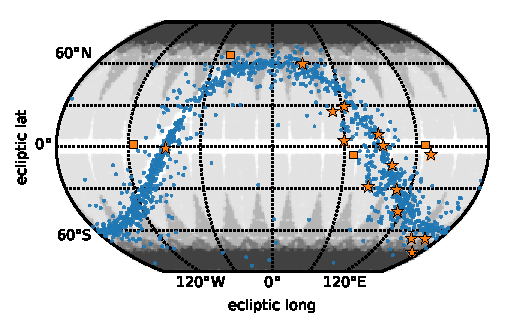
\includegraphics[width=0.7\textwidth]{f1_PLACEHOLDER.pdf}
	\end{center}
	\vspace{-0.5cm}
	\caption{
    {\bf There are many clusters; TESS looks at them.} Placeholder skymap.
		\label{fig:clustermap}
	}
\end{figure*}


%%%%%%%%%%%%%%%%%%%%%%%%%%%%%%%%%%%%%%%%%%
\section{Method: Star Selection}
\label{sec:starselection}

A major motivator for the CDIPS project is to increase the number of
cluster stars for which continuous photometric timeseries are
available, and thus facilitate studies of exoplanetary and stellar
processes across different times and stellar environments.

An essential aspect of the project is therefore to define a {\it
cluster star sample}, consisting of stars that are thought to be
members of clusters.

Performing a homogeneous membership determination for every known
cluster is beyond the scope of this work.  Instead, we collect various
cluster membership catalogs from the literature.  We then use them to
identify cluster members for which we have already made lightcurves
from the TESS images.  Our goal in selecting stars is completeness,
rather than precision.  If there has been a claim in the literature
that a star should be considered as a cluster member, we aim to
provide a lightcurve for that star.

Table~N describes the cluster membership catalogs we have used to
identify candidate cluster members.  Since our photometric reduction
is based on positions reported in {\it Gaia DR2}, each of our
lightcurve sources by default is associated with a Gaia identifier.
Correspondingly, the cluster membership determinations performed by
\citet{cantat-gaudin_gaia_2018} and \citet{gaia_hr_2018} are the
easiest case for us to merge against our lightcurve database.
For the TESS Sectors 1--5 lightcurves produced in this study, this
yielded X and Y lightcurves respectively.



%FIXME: make table

\subsection{Open clusters (OCs)}
\label{subsec:oc}

\paragraph{{\it Gaia}-derived OC memberships}
At the time of writing, two relatively large, homogeneous cluster
memberships studies had been performed using {\it Gaia}-DR2: those by
\citet{cantat-gaudin_gaia_2018} and \citet{gaia_hr_2018}.

\citet{cantat-gaudin_gaia_2018} used an unsupervised membership
assignment algorithm to identify clusters in the three-dimensional
astrometric space of proper motion and parallax. They used {\it Gaia}
photometry and radial velocities to then verify the claimed
membership properties.  From their Table~2, we collect 401{,}448
cluster members, in 1229 clusters, down to a limiting magnitude of
$G=18$.

\citet{gaia_hr_2018} reported memberships for stars in a smaller, more
select group of well-studied open clusters. From their Table~A1, we
collect 40{,}903 cluster members, in 41 open clusters, mostly within
$500\,{\rm pc}$. While this work also included memberships for
globular clusters, we omitted these from consideration.


\paragraph{Pre-{\it Gaia} OC memberships}
\citet{Kharchenko_et_al_2013} used proper motions calculated in PPMXL
\citep[][a combination of USNO-B1{.}0 and 2MASS
astrometry]{roeser_ppmxl_2010} and near-infrared photometry from 2MASS
\citep{skrutskie_tmass_2006} and reported the existence of 2859 open
clusters and stellar associations.
We selected their ``$1\sigma$'' members according to the
combined photometric, kinematic, and spatial criteria described by
\citet{kharchenko_global_2012}.  Then, to obtain {\it Gaia}-DR2 source
identifiers for the members, we performed a crossmatch for {\it
Gaia}-DR2 sources within 5 arcseconds of the listed positions.  As an
additional constraint, we used the 2MASS photometry to predict the
$G$-band magnitudes\footnote{See
\url{https://gea.esac.esa.int/archive/documentation/GDR2/Data_processing/chap_cu5pho/sec_cu5pho_calibr/ssec_cu5pho_PhotTransf.html},
online, \texttt{2019-03-29}, or \citet{carrasco_gaia_2016}}, and
required that the measured $G$-magnitude fall within 2 magnitudes of
the predicted $G$-magnitude.  If multiple neighbors matched the
position and magnitude constraints, we took the nearest spatial
neighbor as the match.  From 373{,}226 stars, this yielded a unique
best neighbor for 352{,}332 stars (94.4\% of the sample), and a choice
between two neighbors for 17{,}774 stars. 

The second (non-{\it Gaia} derived) open cluster membership catalog we
used was the \citet{dias_proper_2014} catalog, which was based on
UCAC4 proper motions.
From their 1805 reported open clusters, we selected sources with
quoted membership probability above 50\%.
To obtain {\it Gaia}-DR2 source identifiers for the members, we
performed a similar crossmatch as before, looking for sources within 5
arcseconds of the listed positions, and within $\pm$2 $G$-band
magnitudes of the prediction.
From 2{,}034{,}269 stars, this yielded a unique
best neighbor for 1{,}828{,}630 stars (89.9\% of the sample), and a choice
between two neighbors for 8.7\% of the remaining sample. 

\begin{figure*}[!ht]
  \gridline{\fig{f5a.png}{0.95\textwidth}{}}
  \vspace{-0.8cm}
  \gridline{\fig{f5b.png}{0.95\textwidth}{}}
  \caption{
      {\it Top.} Cross-match statistics from \cite{Kharchenko_et_al_2013} {\it 
      vs.} Gaia-DR2.
      {\it Bottom.} Ditto, for \cite{dias_proper_2014} {\it vs.} Gaia-DR2.
  }
  \label{fig:xmatch_info}
\end{figure*}

The distributions of various cross-matching statistics are shown in
Figure~\ref{fig:xmatch_info}.  The distances between matches is
typically below 1 arcsecond.  The Dias catalog shows somewhat stronger
crowding effects at the faint end compared to the Kharchenko catalog.
The Kharchenko catalog also has a more lop-sided distribution of true
{\it vs.} predicted $G$-band magnitudes.


\subsection{Moving groups and stellar associations}
\label{subsec:mg}

Stars, moving groups and stellar associations are of interest for
similar reasons as stars in open clusters.  Though fewer stars
are known to exist in moving groups, they are of particular interest
because moving groups are less crowded than open clusters, and are
often closer to the Sun.

We obtained Gaia DR2 identifiers from the results of the following
studies:
\citet{gagne_banyan_XI_2018},
\citet{gagne_banyan_XII_2018},
\citet{gagne_banyan_XIII_2018},
\citet{kraus_tucanahor_2014},
\citet{roser_deep_2011}, % OC, not MG...
\citet{bell_32ori_2017},
\citet{rizzuto_multidimensional_2011},
and \citet{oh_comoving_2017}, The methods applied in these studies
vary from kinematic analyses, to astrometric analyses included
Gaia-DR1 parallaxes, to photometric searches for infrared excesses, to
spectroscopic studies including RVs, H$\alpha$
emission, and Li absorption.

For the Gagne et al{.} catalogs, we searched the Gaia-DR2 archive for
sources within 10 arcseconds of the listed positions.  If Gagne et
al{.} gave a proper motion, we required that the sign of each the Gaia
proper motion components match that of the Gagne values (the stated
proper motion uncertainties seemed to have been underestimated).  We
also imposed a $G<18$ cut on any putative matches.  Of 3012 moving
group members collected from the three combined Gagne et al{.}
catalogs, we found 2702 matches.

The \citet{kraus_tucanahor_2014}, \citet{roser_deep_2011}, and
\citet{bell_32ori_2017} studies reported members in Tucana-Horologium,
the Hyades, and 32$\,$Ori respectively.  Applying the same procedure as
for the Gagne catalogs gave 187, 684, and 119 best-neighbors
respectively, compared to 205, 724, and 141 initially reported
members.  Note that \citet{kraus_tucanahor_2014} found that only
$\sim$70\% of their listed members have spectroscopic indicators
consistent with their membership in Tucana-Horologium.

\citet{rizzuto_multidimensional_2011} also focused on a single moving
group: the Sco OB2 association. We used their reported Hipparcos
identifiers, and matched against the {\it Gaia} archive's
\texttt{hipparcos2\_best\_neighbour} table, which gave 319
nearest-neigbor stars from 436 candidate members.

Finally, \citet{oh_comoving_2017} searched for comoving stars in the
$\approx$2 million stars that overlapped between Tycho-2 and {\it
Gaia}-DR1.  They found many wide binaries, and also identified a large
number of comoving groups.  We chose the 2{,}134 stars that they
reported were in groups with sizes of at least 3 stars.  Using their
{\it Gaia}-DR1 source identifiers, we matched against the {\it Gaia}
archive's \texttt{dr1\_neighbourhood} table, which gave 1{,}881
nearest-neigbor stars in groups of at least three stars
\citep{marrese_gaia_2019}.

\subsection{Summary of selected stars}

After collecting the results of all the studies described above, we
merged them into a single table. We queried the
\texttt{gaiadr2.gaia\_source} table to retrieve their photometric $G$,
$G_{\rm R_p}$, and $G_{\rm B_p}$ magnitudes, as well as their
five astrometric parameters $(\alpha, \delta, \mu_\alpha, \mu_\delta,
\pi)$.
We then imposed that $G_{\rm R_p} < 16$.
The concatenated results are given in Table~N.

All told, there are 1{,}308{,}706 unique stars, from 12 distinct
membership catalogs.
Stars that are reported in multiple catalogs have their reference
information from each available catalog concatenated.






%%%%%%%%%%%%%%%%%%%%%%%%%%%%%%%%%%%%%%%%%%
\section{Method: Photometry}
\label{sec:method}

\begin{figure}[t]
	\begin{center}
		\leavevmode
		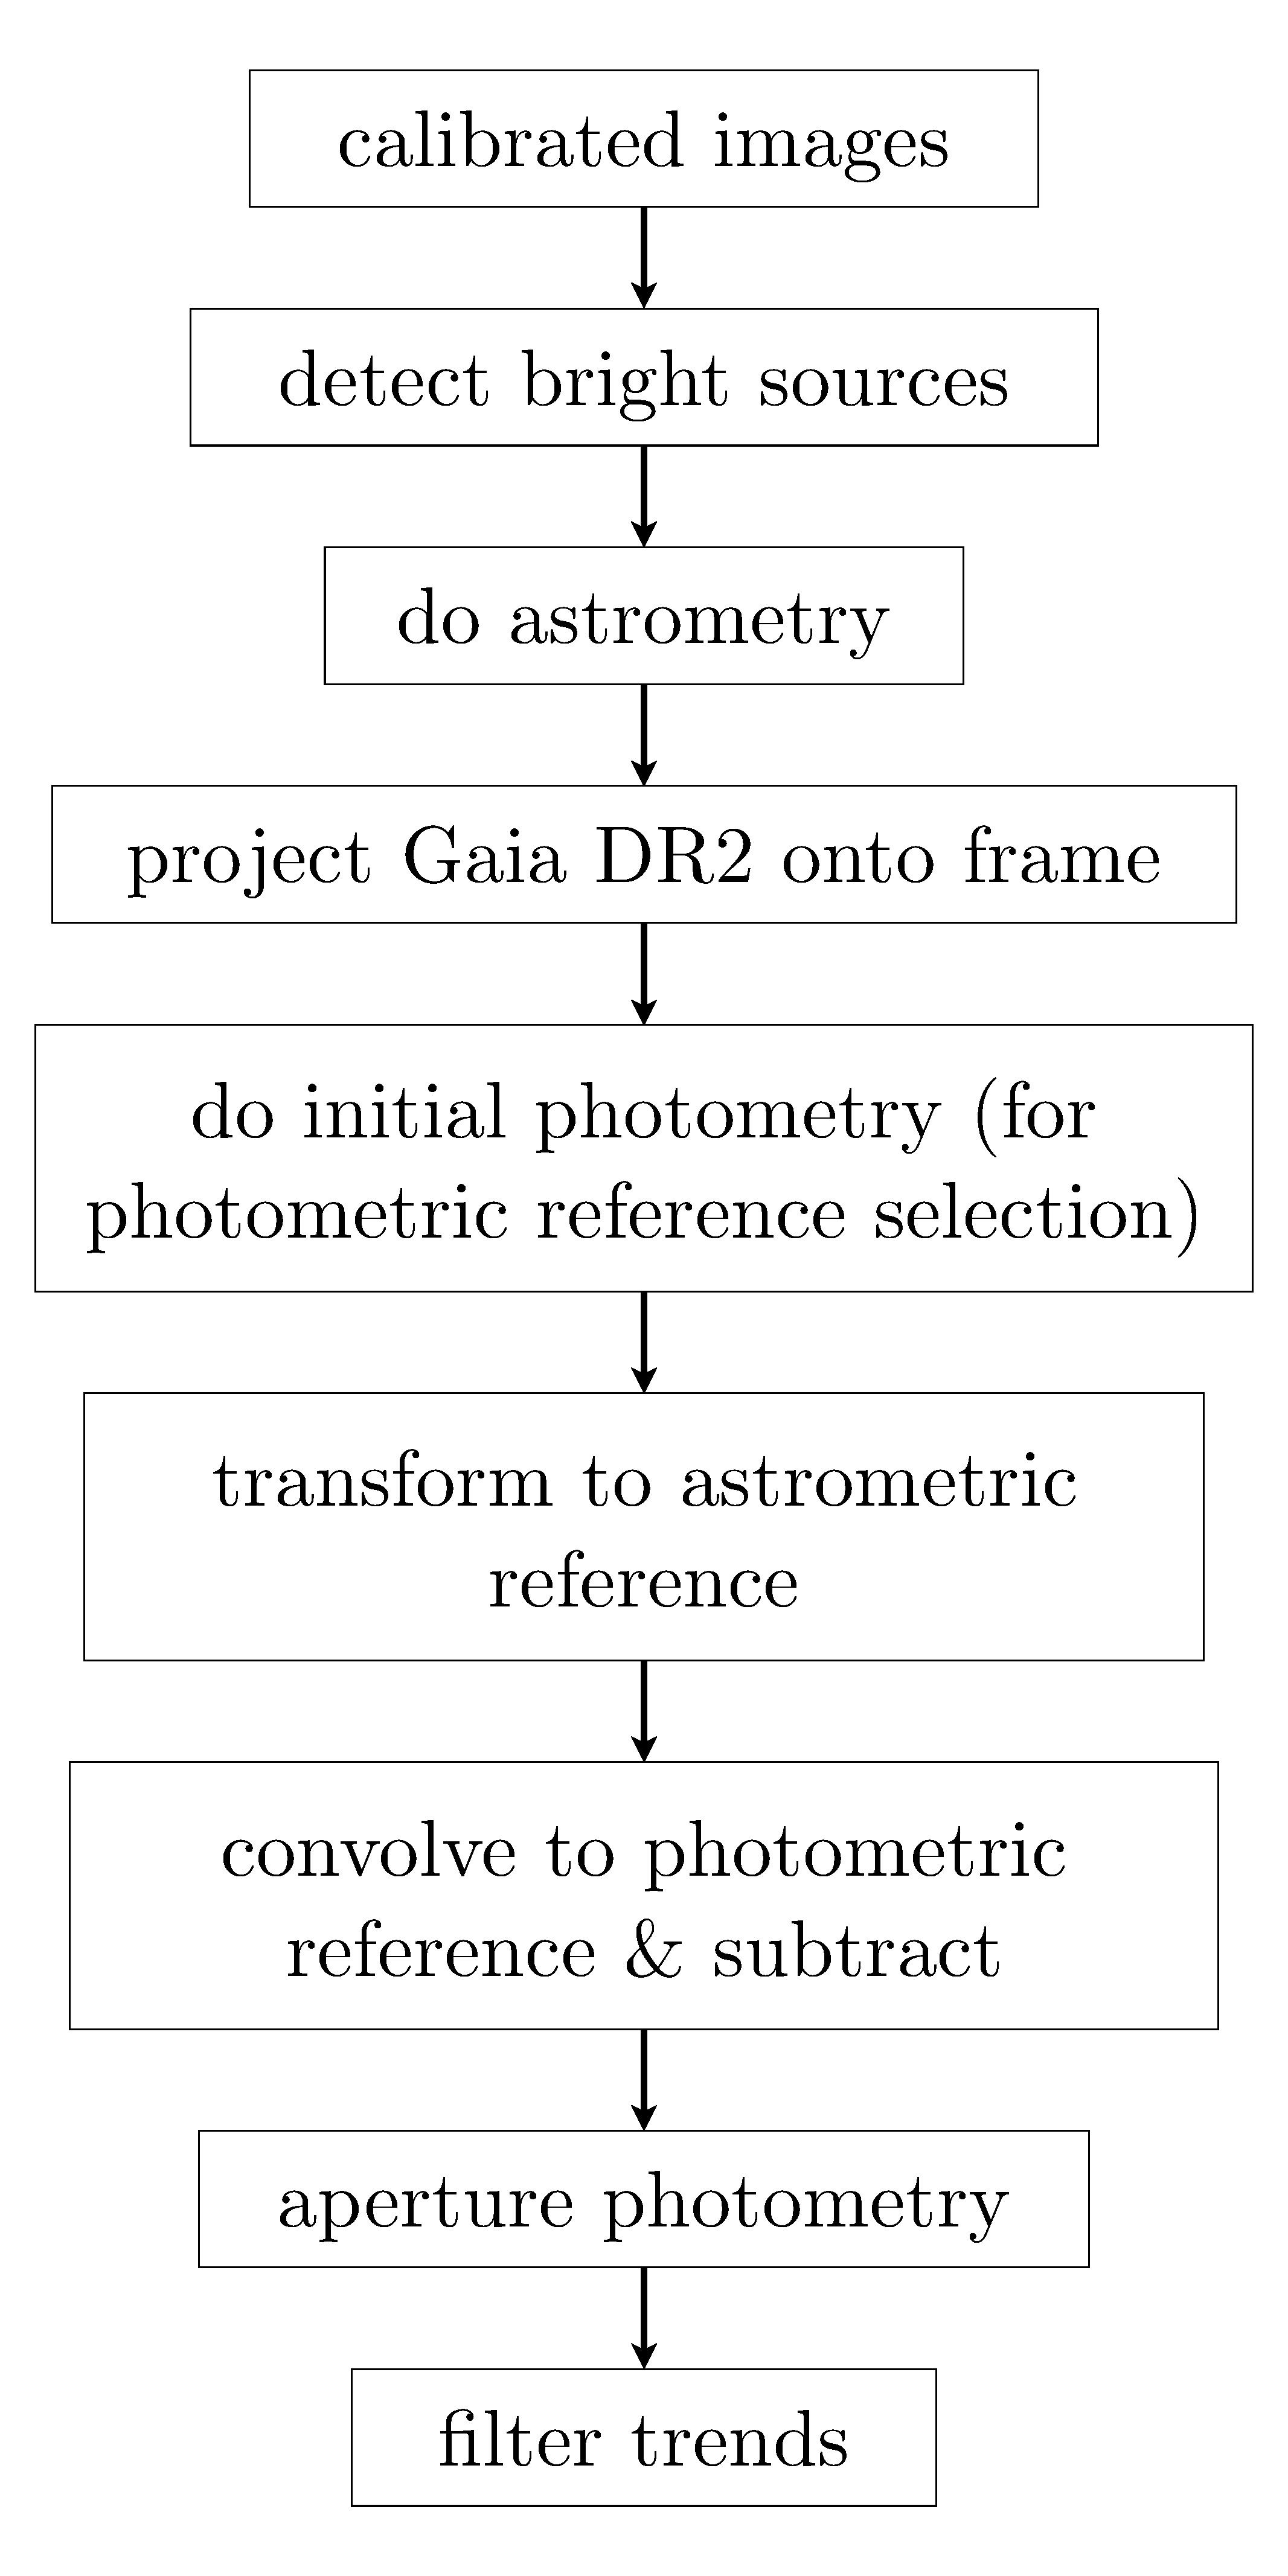
\includegraphics[width=0.3\textwidth]{f2.pdf}
	\end{center}
	\vspace{-0.5cm}
	\caption{
    {\bf Pipeline.} This is what we do.
		\label{fig:pipeline}
	}
\end{figure}

\subsection{Overview}

We reduced the TESS images to lightcurves by performing a sequence of
steps using stand-alone programs.  A conceptual overview of our
``pipeline'' is given in Figure~\ref{fig:pipeline}.  
Our overall method is in the spirit of the reduction approaches used
by \citet{Pal_2009}, \citet{soares-furtado_image_2017} and
\citet{oelkers_precision_2018}.

We begin with the calibrated full frame images produced by SPOC
(\S~\ref{subsec:observations}).  We then perform a collection of
preparatory steps, including source extraction of bright stars,
astrometry using the resulting positions, and coarse simple aperture
photometry (\S~\ref{subsec:preparation}).  Using the shape values from
the initial astrometry, we select an astrometric reference frame and
transform all of the calibrated images to it.  We construct a
photometric reference by stacking a collection of frames, and then
convolve all the transformed frames to the photometric reference,
and subtract (\S~\ref{subsec:imagesubtraction}).  We perform aperture
photometry on the subtracted images using positions projected onto the
frame from Gaia DR2.  We detrend the resulting lightcurves
(\S~\ref{subsec:lcdetrending}).
We then select stars that we believe are ``cluster members'',
roughly X\% of the overall dataset (\S~\ref{sec:starselection}).
Focusing on the lightcurves of these stars, their white noise and red
noise properties, and point out a few interesting cases of
variability (\S~\ref{sec:results}).




\subsection{Observations}
\label{subsec:observations}

% How did TESS observe?
% What processing steps happened in order to get the calibrated frames?
% Why did we choose to start with them?

The TESS spacecraft began science operations on July 25, 2018.  To
keep its cameras pointed opposite the Sun, the spacecraft advances by
$\approx$$28$ degrees in ecliptic longitude every lunar month.  Data
acquired throughout each ``sector'' are downlinked at spacecraft
perigee through the Deep Space Network.  Verbose descriptions of the
spacecraft's design and operations are given by
\citet{ricker_transiting_2015} and the instrument handbook
\citep{vanderspek_2018}.

For us, the main data product of interest is the calibrated full frame
image (FFI).  Each TESS camera reads out every 2 seconds.  To produce
a manageable telemetric load, the resulting pixel values are averaged
by the onboard computer into 30 minute exposures. An on-board cosmic
ray mitigation algorithm is applied (CITE: BERTA-THOMPSON). Once
transmitted to the ground, the raw images are calibrated by the
Science Processing Operations Center.  The calibration process
includes an overscan, bias, and dark current correction, and also
divides out a flat field.  The details are given by
\citet{clarke_kepler_2017}, and the resulting science data products
are described by \citet{tess_data_product_description_2018}.

We begin our analysis using the calibrated images, their uncertainty
maps, and their associated headers.  The spacecraft has four cameras,
and each camera has four CCDs.  In the following analysis, all
image-level operations are thus performed on the images for each CCD,
so that at any instant of time there are 16 independent images
undergoing analysis.


\subsection{Image Preparation \& Background Removal}
\label{subsec:preparation}

Before we can perform any kind of photometry, a few janitorial tasks
are required.

First, we trim the images.  We convert the calibrated image from MAST
into a single-extension FITS image, trimmed to remove virtual rows and
columns using the \texttt{SCIROWS}, \texttt{SCIROWE}, \texttt{SCCSA},
and \texttt{SCCED} header values.

We then estimate the background of each frame.  We do this by
temporarily masking out pixels more than $2\sigma$ from the median,
and then passing a $48\times48$ median box filter over each pixel in
the image, using reflective boundary conditions. We subtract out this
smooth background estimate from each image.  This step helps mitigate
two unwanted image artifacts.  First, it removes a low-level glow
present in the corners of many images, which remains even after
flat-fielding \citep[see][\S 7.3.5]{vanderspek_2018}.  Second,
background subtraction removes scattered light patches from the Earth
and Moon, which vary in positions around the camera boresight over
each spacecraft orbit \citep[see][\S 7.3.1--7.3.4]{vanderspek_2018}.
The typical size of scattered light patches is greater than 48 pixels,
and their typical amplitude is $\sim 10\times$ the sky background
level. 

% We found this background subtraction step to be particularly important
% in our subsequent difference imaging analysis. In its absense, the
% scattered light artifacts could introduce erroneous residuals into the
% kernel solution used to match reference and target images.  Including
% this step mitigated such effects, and helped produce clean
% subtractions.  Even after subtraction, a small fraction of frames also
% show sharp features (caustics) below our median box filter's size
% scale.  Such features may affect flux measurements at specific times
% in a small subset of lightcurves.

After subtracting the background, we mask out saturated stars using a
fixed saturation level of $8\times10^4\,{\rm ADU}$. This value was
chosen based on the onset of visible trails of bleeding charge, and is
slightly greater than the expected saturation level quoted by
\citet{vanderspek_2018}.  As described by \citet{Pal_2009}, our masks
are metadata to the image, and are only applied to the
pixel values during the specific image processing steps ({\it e.g.},
convolution) in which they are necessary. We also extend the masks
beyond purely saturated pixels to ``bloomed'' pixels horizontally and
vertically adjacent to the saturated pixels using the algorithm
described by \citet{Pal_2009}.

Finally, for frames with the \texttt{DQUALITY} bit-flag corresponding
to the ``momentum dumps'' and ``coarse pointing modes'' described by
\citet{vanderspek_2018}, we mask out the entire frame.  This removes
on average a few frames per sector. Through visual inspection, we see
that the stars on these frames are extremely smeared, and are unlikely
to produce useful science data.
In addition, we use the sector-specific data release
notes\footnote{\url{ archive.stsci.edu/tess/tess_drn.html}} to
identify further  times with anomalously poor spacecraft performance,
which we omit from consideration. For Sectors 1 through 5, these
include coarse pointing windows from orbits 10, 13, 14, and an
instrumetal anomaly window in orbit 15.

Next, we perform some initial analysis steps to produce metadata
needed during image subtraction.  To obtain an astrometric solution
(independent from the WCS data packaged with the frames), we use
\texttt{fistar} to perform source extraction on bright stars in each
image.  We pass the resulting source lists through
\texttt{astrometry.net} \citep{lang_2010}, which returns an
astrometric solution for each frame packaged in the WCS format
\citep[][Sec.~8]{pence_fits_2010}.  During the initial source
extraction, we also fit elongated gaussians to the bright stars,
yielding the shape parameters $(s,d,k)$, where the flux as a function
of position is assumed to take the form
\begin{align}
  f_{\rm elong}(\vec{x}) &= B + A \exp \{ -0.5 \times ( 
    s(\Delta x^2 + \Delta y^2) + \\
    \nonumber
    &d(\Delta x^2 - \Delta y^2) +
    k(2\Delta x \Delta y)
  )  \},
\end{align}
for $\Delta x = x-x_0$, and $\Delta y = y - y_0$.  For a nearly
circular shape profile, the sharpness $s$ is related to the FWHM as
${\rm FWHM} \approx 2.35\sqrt{s}$ \citep[{\it e.g.},][]{Pal_2009}.
These shape parameters are later used when selecting an astrometric
reference (\S~\ref{subsec:imagesubtraction}).  We note that the fast
focal ratio of the TESS cameras introduces significant comatic
aberrations to the images: stars closer to the center of the field are
more round, while stars towards the edges are more triangular.

With the resulting WCS information, we then project a source catalog
from Gaia-DR2 onto the frame, down to a pre-selected magnitude cutoff
\citep{gaia_collaboration_gaia_2018}.  We use these expected positions
to center the apertures in our photometry, rather than attempting to
detect the positions.  Such ``forced-aperture photometry'' is
preferable to performing source extraction because of the large TESS
pixels, and the accurate Gaia positions.  The Gaia-DR2 epoch is
J2015.5, so even the fastest-moving stars with proper motions of
$\sim$$1\,{\rm arcsecond}\,{\rm yr}^{-1}$ are still well within one pixel
of their predicted positions in the TESS images.  The projection and
catalog-indexing is performed using
\texttt{gaia2read}\footnote{\url{github.com/samuelyeewl/gaia2read}}
\citep{kim_2018_gaia2read}.

Finally, we perform aperture photometry on the bright stars from the
source list, by summing the counts inside appropriately-weighted
circular apertures centered on the projected positions from Gaia DR2. 
The pixel weights $w_{x,y}$ are equal to the fraction of the pixel
that falls within the aperture.  They are thus unity for pixels
entirely within the aperture, and fractional along the aperture
boundary (e.g., \citealt{Pal_2009} Fig 17). 
The background levels are measured in annuli around each aperture
center.  The raw flux of the object after background removal is then
(\citealt{Pal_2009} Eq 65)
\begin{equation}
  f = \sum_{x,y} w_{x,y} (I_{x,y} - B) = f_{\rm total} - B r_0^2.
  \label{eq:simple_aperture_phot}
\end{equation}
The resulting measurements, for instance of the background level of
each aperture, and the number of ``good'' objects that are detected,
are later used as input for selecting photometric reference frames.


\subsection{Image Subtraction}
\label{subsec:imagesubtraction}

The core operation of ``classical'' image subtraction
attempts to match a photometric reference $R$ and a target image $I$ by 
computing a convolution kernel.
The kernel, once applied to the high signal-to noise reference,
produces a model image, $M_{xy}$,
\begin{equation}
    M_{xy} = (R \otimes K)_{xy} + B_{xy},
\end{equation}
where $B_{xy}$ is a component of the model image that allows for
background variations.
The convolution kernel $K$ is typically decomposed onto a
basis, $K = \sum_i c_i K_i$, and the coefficients are found
by minimizing
\begin{equation}
    \chi^2 = \sum_{xy} \left( \frac{I_{xy} - M_{xy}}{\sigma_{xy}} \right)^2,
\end{equation}
where $\sigma_{xy}$ is the uncertainty in the target image pixel values.
Photometry is then performed on the difference image $D_{xy}$, where
$D_{xy} = I_{xy} - M_{xy}$.

% FIXME: describe gaussian kernel (used in e.g., KELT, and maybe other 
%pipelines?). Perhaps give Eqns for delta kernel.
The choice of kernel ...



We then select two ``reference frames'' for image subtraction.
The first is the astrometric reference; the second is the photometric
reference.
To choose the astrometric reference, we use the following heuristics:
\begin{enumerate}
  \item The frame must have large and round stars (largest ``S'',
    smallest ``D'' and ``K'' values).
  \item The frame must minimal background noise, as measured in annuli
    around the bright stars selected in \S~\ref{subsec:preparation}.
  \item The frame must have, relative to the other frames being
    considered, a large number of detected sources.
\end{enumerate}
We sort the frames using the above metrics, and then select the
astrometric reference from successive intersections of each sorted
list.
Using the algorithm presented by \citet{pal_astrometry_2006}, we then
calculate a spatial transformation that maps the X and Y coordinates
from each calibrated frame onto the the astrometric reference.

``Registering'' the images onto a common astrometric reference frame
requires some care. In particular, the transformation must preserve
the fluxes of the sources. Since the transformation is affine (a
combination of {\it e.g.}, translation, rotation, dilation, and shear)
standard bilinear or bicubic interpolation would not achieve flux
conservations.  We therefore use the flux-conserving interpolation
scheme described by \citet{Pal_2009} which is based on analytic
integration of the surfaces determined by the pixel values. 
%FIXME: is this interpolation scheme definitely being applied?
The largest component of the transformation is a translation, of order
2 arcseconds, or about 0.1 TESS pixels.

The second reference frame needed for image subtraction is the
photometric reference.  Generically, if one were to simply subtract
two arbitrary frames, the noise level in the resulting difference
image would be $\sqrt{2}$ times greater than that in the original
target frame.
To minimize this effect, we create a high-SNR median average of
$N$ selected frames, so that the noise level in the resulting
subtracted images goes as $\sqrt{1+1/N}$.
This ``photometric reference'' is used both to calculate the
convolution kernel during image subtraction, and to measure the
reference flux of each star.
To select viable frames for inclusion in the photometric reference, we
use the results of our initial photometry step
(\S~\ref{subsec:preparation}), and sort frames for each sector by:
\begin{enumerate}
  \item Lowest median scatter in photometry
  \item Lowest median error in photometry
  \item Lowest median background measurement
  \item Lowest median absolute deviation in background measurements
  \item Largest number of stars detected by \texttt{fiphot} with good
    flags.
    % fiphot files used for all of this.
\end{enumerate}
We convolve the 50 best candidate photometric references to the best
photometric reference, and then perform a median combination of the
frames to make the photometric reference.

%FIXME: it seems like it would be smart to produce a photometric
%reference for different intervals of time. 480 frames over 10 days ->
%perhaps split the full 28 day sector entirely by momentum dumps to
%get ~10 photometric references per sector. 

%FIXME: LEFT OFF HERE
Some details of, and motivation for, the convolution process are warranted.
The general idea of the image subtraction problem is to...

This has some benefits for crowded regions. Most notably, in enables a
measurement of the background flux level.

Our approach follows from the algorithm presented by
\citet{Alard_Lupton_1998}, and explained in detail by
\citet{miller_optimal_2008}.
The process is: %FIXME: following miller 2008...
\begin{enumerate}
  \item Select a set of isolated stars (``stamps'').
  (For ficonv, the default procedure is: grid up the image. Within
    each grid... find the brightest nonsaturated region. Use that to
    fit the kernel!)
  \item Choose basis vectors $K_n$ for the kernel, $K = \sum_{n=1}^N
    a_n K_n$. Our goal is to determine the best-fitting coefficients
    $a_n$. 
  \item Using these stamps and the least-squares method, ...
\end{enumerate}


%FIXME: when do we actually get the reference fluxes? Where do those
%come from???

Finally, we convolve and subtract all the frames that have been
translated from the photometric reference (\texttt{grcombine}).
We use the same kernel formalism as described by
\citet{soares-furtado_image_2017}.
To compute the convolution kernel, we minimize the difference between
each image and the photometric reference (or something like this),
using the Alard \& Lupton 1998 method (CITE, also CITE Miller's
reference).
The software implementation is that by \citet{Pal_2009}, in the
\texttt{ficonv} program.
The implemented math is as follows.
\begin{equation}
  XXX = XXX. %FIXME: maybe Soares pg 5 main equation?
\end{equation}
We explored a variety of kernel options, including X, Y, and Z.
We wound up including an ``identity'' term (MEANING?), a ``background
term'' (MEANING?) and a delta function term (MEANING? Give math for
all of these).
There are also spatially-varying terms of order XX. (MEANING?)
% I believe this means that we should be able to somehow _visualize_
% the kernel as a function of spatial position in the image. What
% should it look like? Is it like a star's PSF? Or somehow related??

We perform forced-aperture photometry on the subtracted frames,
using the locations from the Gaia projection, to measure the resulting
difference fluxes.
We use circular apertures, with the appropriate weigths along the
boundaries (\texttt{fiphot}; \citet{Pal_2009} Section FIXME).

Note that to measure the fluxes on the differenced images, a
slightly different procedure from Eq.~\ref{eq:simple_aperture_phot} is
relevant.
(Pal 2009 Section 2.9).
Specifically, the subtracted image $S$ is given by $I - B - R\ast K$,
for $I$ the original image, $B$ the background, $R$ the reference
image, and $K$ the convolution kernel.
The flux in the original image is given by
%FIXME: this equation IS PROBABLY WRONG. I_xy? Or S_xy?
\begin{align}
  f &= \sum_{x,y} w_{x,y} I_{x,y} \\
    &= 
       \frac{1}{|| K ||_1^2} \sum_{x,y} S_{x,y} (w \ast K)_{x,y}
       +
       \sum_{x,y} R_{x,y} w_{x,y},
\end{align}
%FIXME: derive this equation. why exactly does this work?

Finally, to convert from a list of sources on each frame to a list of
flux values at any given time, we use the \texttt{grcollect}
transposition tool.

\subsection{Lightcurve Detrending}
\label{subsec:lcdetrending}

The preceding steps produce lightcurves that include both instrumental
systematics as well as astrophysical variability.  The detrending
philosophy adopted by the HAT group typically proceeeds in two
sequential stages (see discussions from {\it e.g.}
\citealt{bakos_2010,huang_high-precision_2015,zhang_precision_2016}) .
The first stage is to decorrelate against external parameters that are
known to affect the stellar flux measurements (EPD,
\citealt{bakos_2010}). The second stage is to filter remaining
systematic trends caused by unknown parameters by decorrelating the
measured brightnesses of stars against each other (TFA,
\citealt{kovacs_trend_2005}).  

%FIXME TURGID PROSE
In general though, one must adapt detrending procedures to the data at
hand.  In \S~\ref{sec:flux_vs_external_parameters}, we show that the
``external parameter'' dependence visible in the TESS data is rather
complex: ordinary linear model-fitting, as well as an initial attempts
at non-linear model fitting, are poor descriptions of the data.  We go
on to show (\S~\ref{sec:tfa_is_good_enough}) that a plausible
detrending approach for the purpose of transit discovery is to simply
decorrelate against other nearby stars with standard TFA.


\subsubsection{Flux versus external parameters}
\label{sec:flux_vs_external_parameters}

\begin{figure*}[t]
	\begin{center}
		\leavevmode
		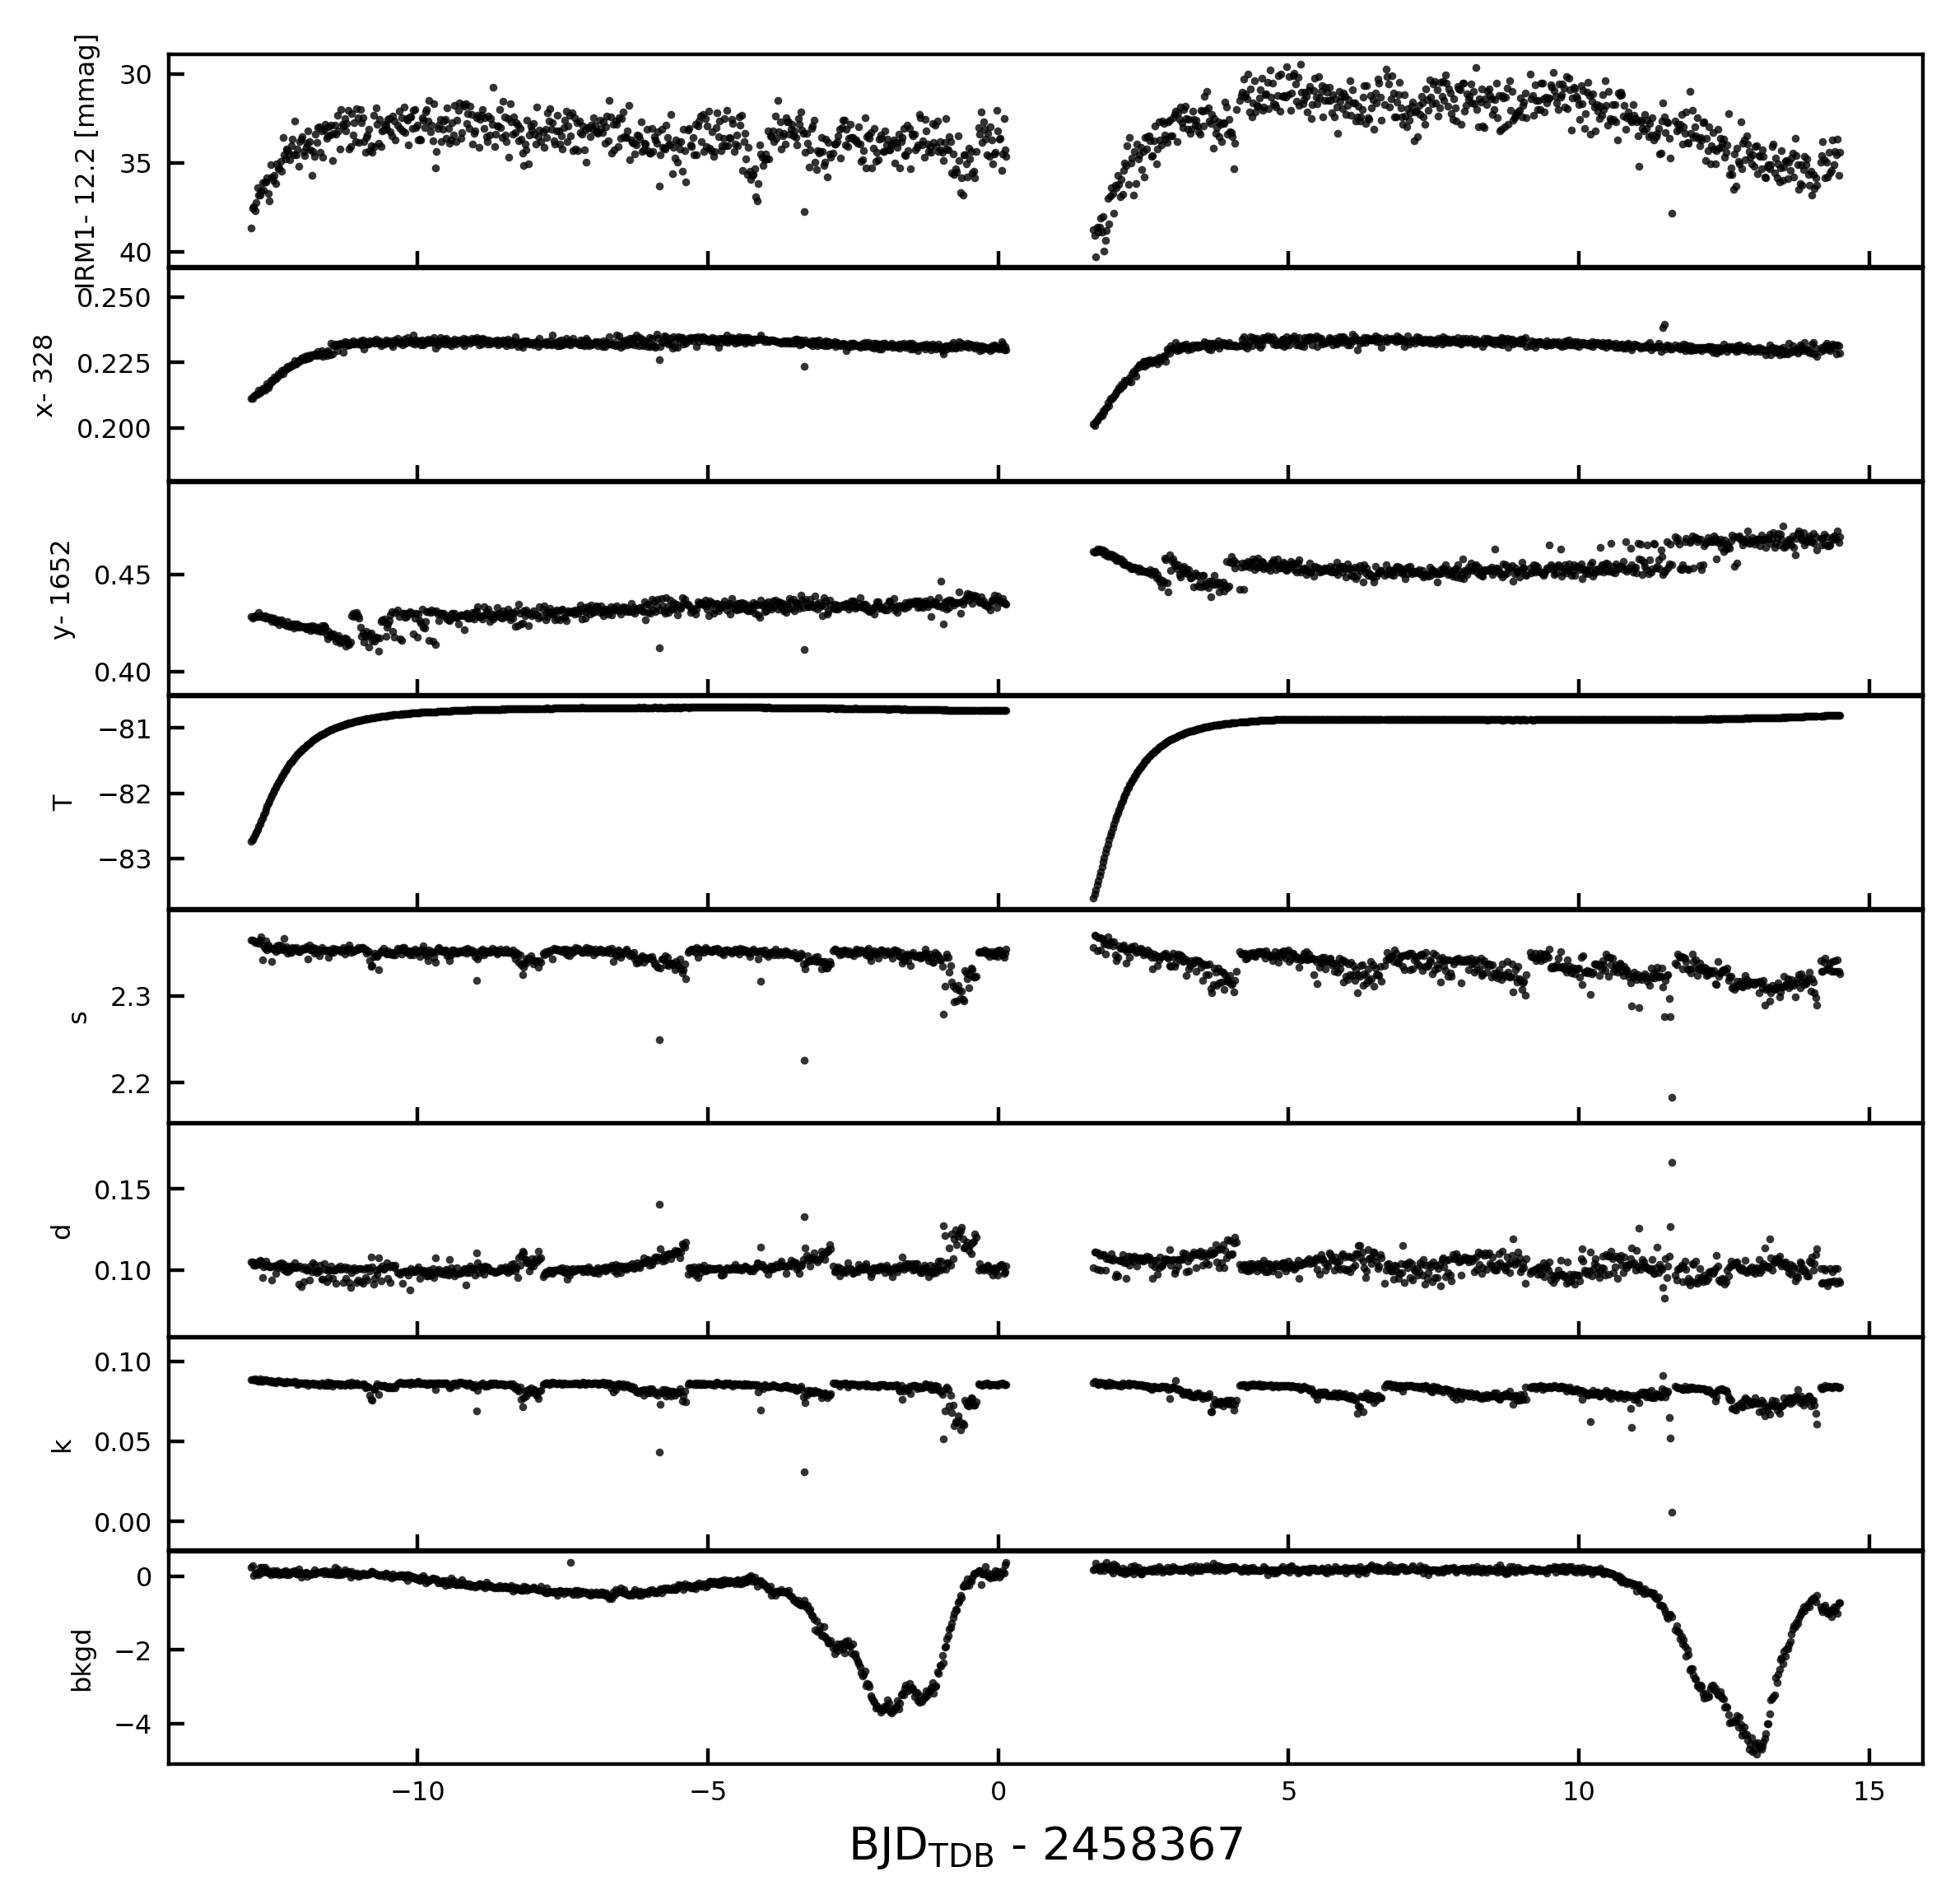
\includegraphics[width=0.7\textwidth]{f3.png}
	\end{center}
	\vspace{-0.5cm}
	\caption{
    {\bf Timeseries of ``external parameters'' for a representative
    star.} {\it Top}: Instrumental raw magnitude (with a particular
    aperture size), as a function of time.  {\it Second and third from
    top}: $x$ and $y$ centroid positions as a function of time.
    Continuing in order are the CCD temperature, the $(s,d,k)$ shape
    parameters, and the measured background value.
    Most of the apparent variability is instrumental: see
    \S~\ref{sec:flux_vs_external_parameters}.
		\label{fig:external_parameter_timeseries}
	}
\end{figure*}


\begin{figure*}[t]
    \begin{center}
		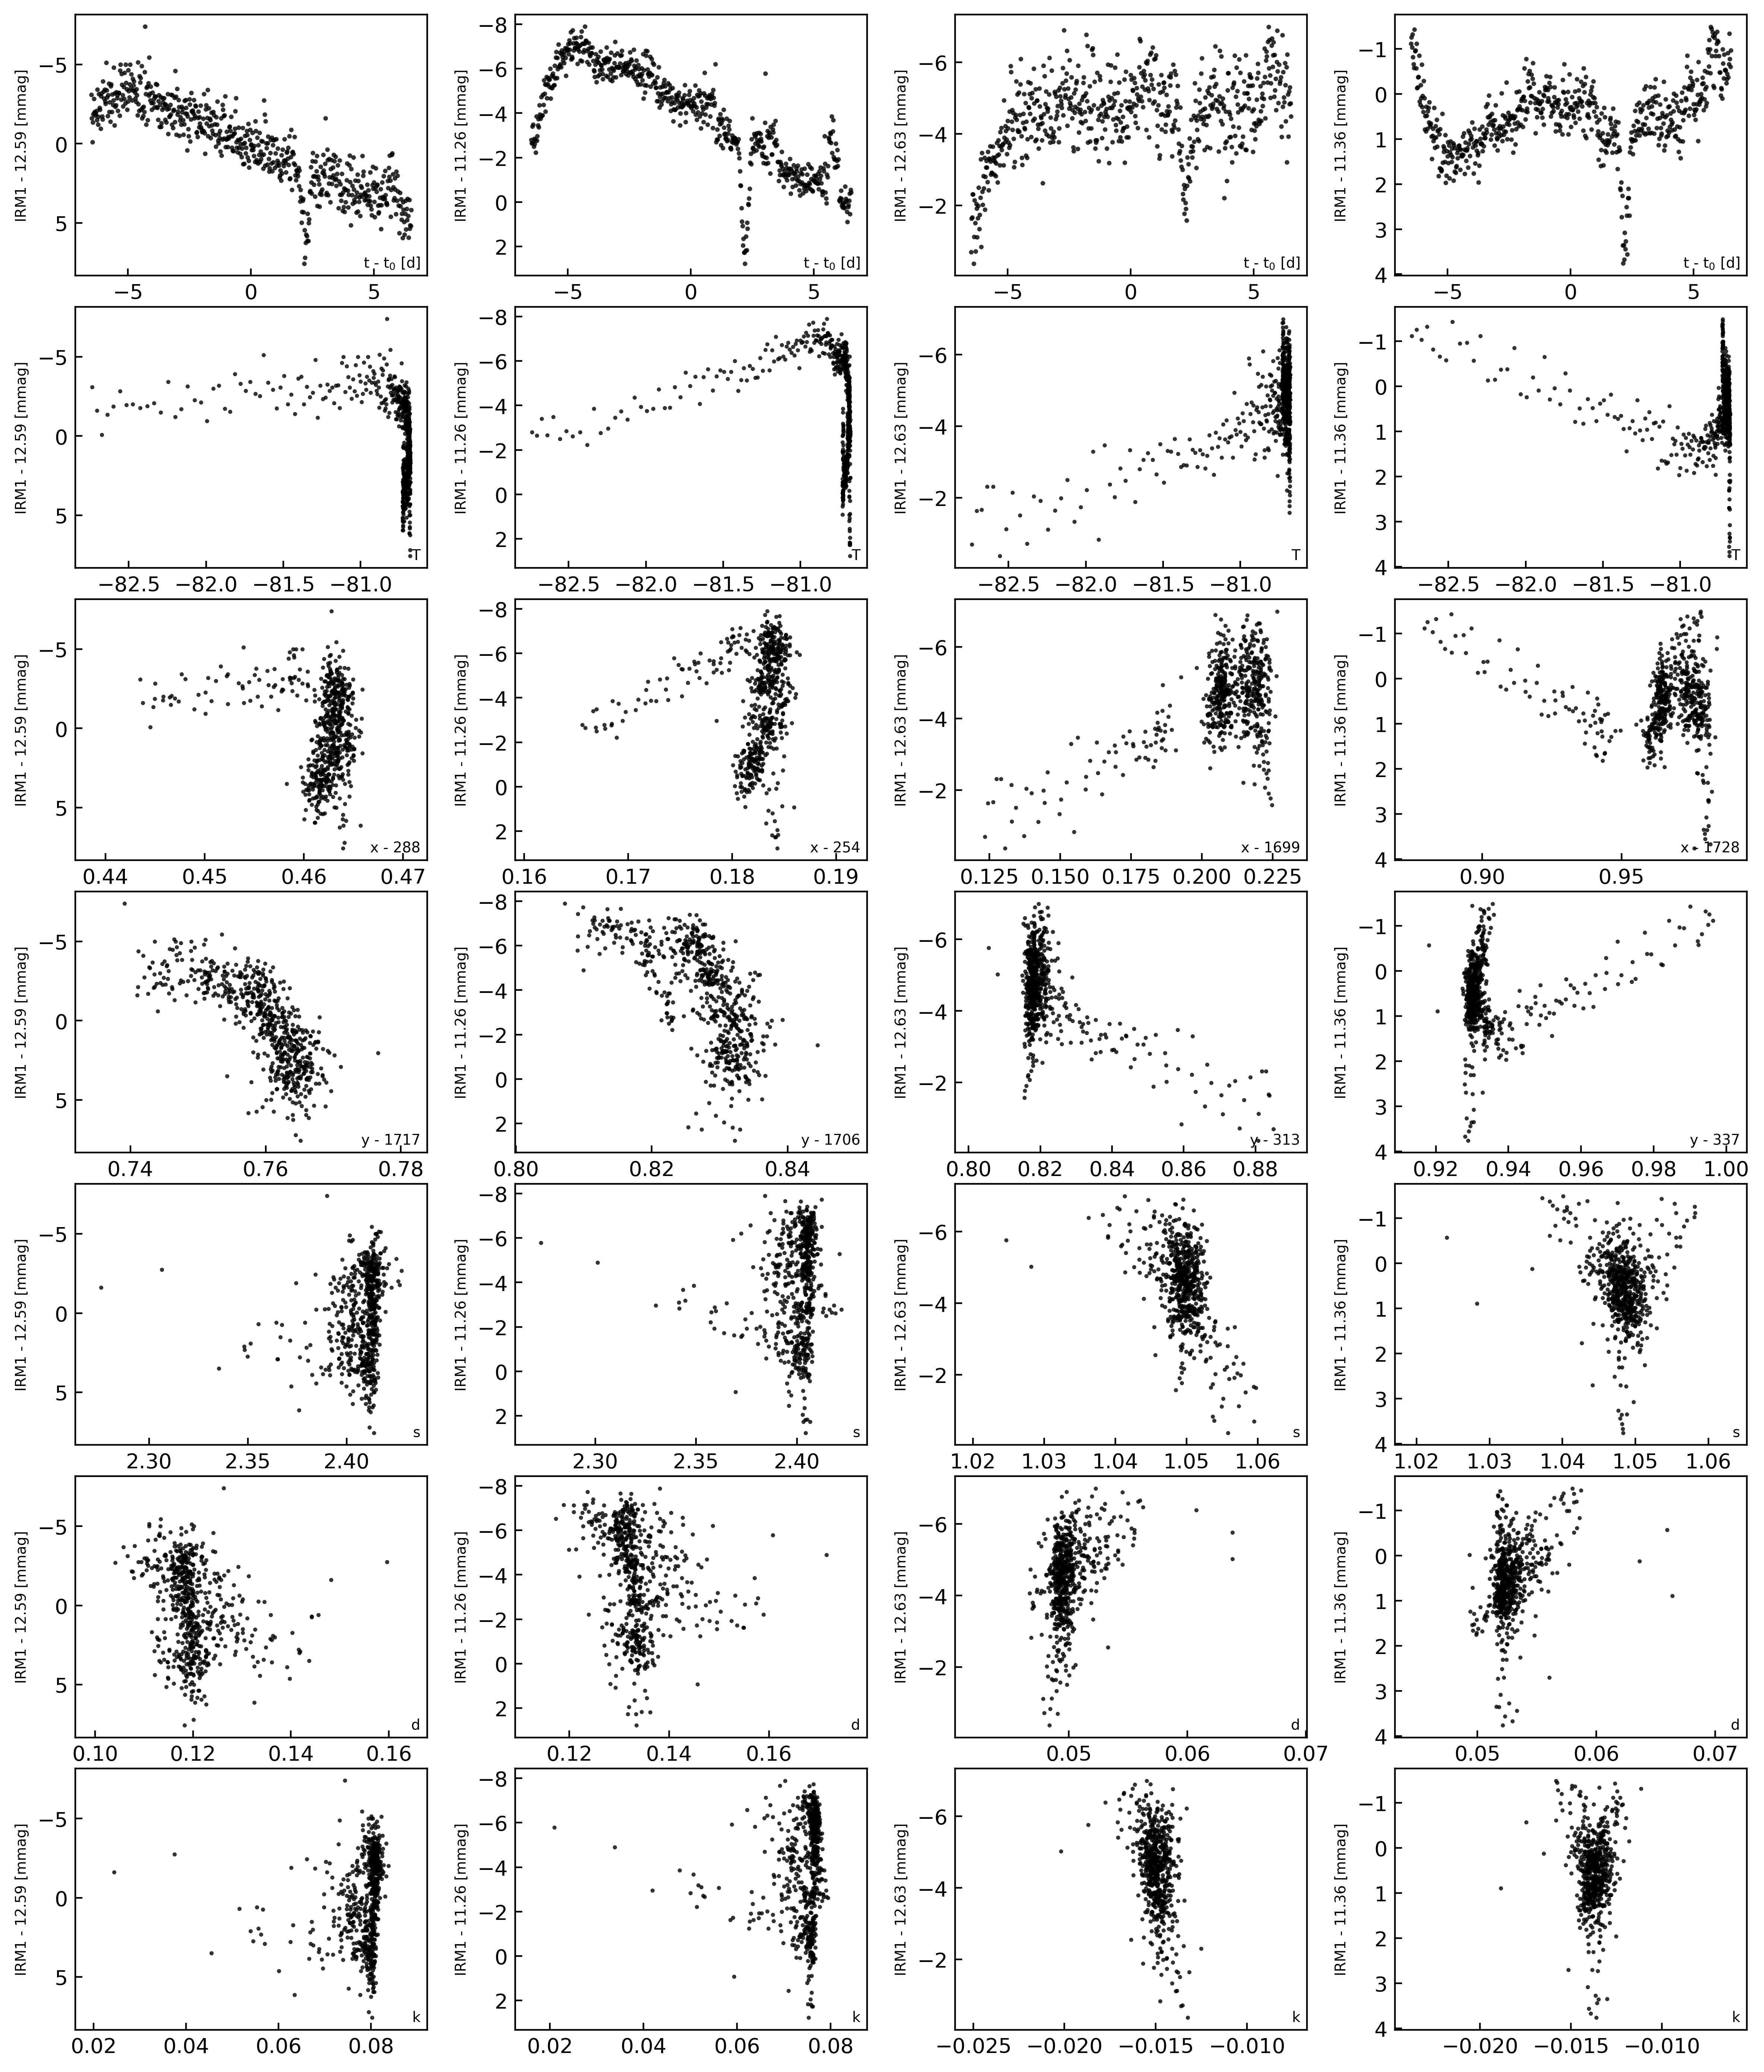
\includegraphics[height=0.95\textheight]{f4.png}
    \end{center}
    \vspace{-0.8cm}
    \caption{
      {\bf Flux as a function of ``external parameters'' for four
      representative stars.} The left two columns are stars at the
      corner of a camera's field; the right two columns are from the
      centers.
      Each row shows a different parameter along the $x$-axis, given
      in text at the bottom right of each subplot.
      ``Hooks'' are common features in flux as a function of
      temperature and centroid position.
      \S~\ref{sec:flux_vs_external_parameters} gives a verbose
      description.
     \label{fig:flux_vs_external_parameters}
    }
\end{figure*}

The traditional approach to EPD 
\citep[][]{Pal_2009,bakos_2010,zhang_precision_2016} is to fit and
subtract a model for the magnitudes $m$ of the form

\begin{equation}
  m = {\rm const.} + \sum_i c_i \theta_i,
  \label{eq:classical_EPD}
\end{equation}

where $\vec{\theta}$ is a vector of parameters such as the shape
parameters $(s,d,k)$, their products $(s^2, s\cdot d, d^2, \ldots)$,
the temperature $T$ of the instrument or environment\footnote{ We used
the temperature from the on-chip aluminum-copper sensor measurements
included in the engineering
data\footnote{\url{archive.stsci.edu/missions/tess/engineering/}}.  },
the centroid positions $(x,y)$, the fractional part of the
centroid positions $(\{x\},\{y\})$, and any other parameters that are
expected\footnote{ The fractional centroid positions might matter
because intra-pixel quantum efficiency variations could affect the
measured stellar brightness.  The varying temperature $T$ of the CCD
electronics might matter.  } to correlate strongly with the observed
flux.  The coefficients $c_i$ are calculated through linear
least-squares, and subtracted to produce ``EPD'' lightcurves.

The premise of this model is that the correlations between the
magnitudes and the external parameters are linear.  For ground-based
CCD data (e.g., HATNet, HATS, and Nikon DSLRs), \citet{bakos_2010} and
\citet{zhang_precision_2016} have verified that this model is a
reasonable description to the data.

To discern whether such a model extends to the TESS data, we examined
scatter plots of each parameter, as a function of all the other
parameters.  We also examined plots of each parameter as a function of
time.  A few prominent trends were present.

\begin{enumerate}

\item {\it Flux vs. time}. Most of the lightcurves we examined showed a secular
    drift with amplitude $0.01\,{\rm mag}$ over the timescale of each
    orbit.  Sharper trends (``hooks'') at the beginning of each orbit
    seemed to be less prominent for stars at the corners of the fields
    than stars at the center.  The periodicity incurred by the
    2.5$\,{\rm day}$ momentum dumps was also noticeable in more of the
    lightcurves at the center of the field than at the corners.

\item {\it Flux vs. centroid positions}. The flux as a function of
  centroid position often showed non-linear ``hooks'' (see Figure
    \ref{fig:flux_vs_external_parameters}). Most of the data points from a 
    given orbit reside at a given
    level, but about 10\% are in a tail. This was seen in lightcurves
    all across the TESS field of view.

\item {\it Flux vs. temperature} exhibited similar hooks, with most of
  the flux values residing at a particular level, and perhaps 10\%
    following a non-linear path (often resembling the Nike ``swoosh'')
    away from the bulk of points.

\item {\it Flux vs. shape parameters}.  For lightcurves in the corner
  of the field of view, similar hooks are present in flux {\it vs.}
    $(s,d,k)$, though the hooks are less sharp.  In the center of the
    field of view, gaussian ellipses are a better description of the
    flux {\it vs.} the shape parameters.
    
\end{enumerate}

Considering the timeseries of parameters other than flux 
(Figure~\ref{fig:external_parameter_timeseries}):

\begin{enumerate}

\item {\it Centroid positions vs. time}.  The main variability in the
  centroid positions as a function of time is a secular drift, that is
    reset every orbit.  The 2.5 day momentum wheel dump is
    superimposed on this secular drift, and has smaller amplitude than
    the drift.

\item {\it Temperature vs. time}.  The main variability in temperature
  {\it vs.} time is a secular drift of the same timescale as that for
    the centroid positions timeseries.

\item {\it Shape parameters vs. time}.  The main variability in the
  shape parameters as a function of time is the 2.5 day momentum wheel
    dump periodicity, with hooks before each momentum dump.

\item {\it Background value vs. time}.  The background is typically stable, 
except when scattered light from the Earth or Moon enters the frame (visible 
towards the end of each orbit in 
Figure~\ref{fig:external_parameter_timeseries}).

\end{enumerate}

Given the characteristics of the variability, a linear model of the
form given in Equation~\ref{eq:classical_EPD} is not applicable.  To
fit out the correlations between flux and parameters which most
commonly exhibited ``hooks'', we explored fitting a parametric open
curve (an $N$-dimensional B-spline, \citealt{dierckx_curve_1996}) to
the flux, centroid positions, and temperatures simultaneously.  We
selected the number of knots through brute-force, by calculating
$\chi^2$ for the model fit over a grid of possible knots, and
minimizing the Bayesian Information Criterion.  Though this approach
showed some initial promise, even with ``optimal'' knot-selection (in
the BIC sense) it introduced undesirable residuals in the lightcurves,
and also distorted transits.

Given these complications, for the time being we omit the step of
``detrending'' as a function of external parameters. To
enable further exploration of the issue, we include all the necessary
vectors of {\it e.g.}, centroid positions, temperatures, and shape
parameters in our reported lightcurves.



\subsubsection{Trend filtering algorithm}
\label{sec:tfa_is_good_enough}


Since most of the external parameter dependence is shared between
stars, we opt to decorrelate the flux timeseries of each star
against other stars in the frame (TFA, \citealt{kovacs_trend_2005}).

%TODO: write out the procedure, give a model equation!

This requires selecting ``template stars'', which are a subsample of
star that are supposed to represent all the types of systematics
across the dataset. 
%FIXME: clarify this procedure
We select XXX template stars randomly from the stars on-chip with
$G_{\rm R_p}$ magnitudes between 8.5 and 13 (TODO: rather bright?).
As an initial variability cut, we fit a parabola in the RMS-magnitude
plane, and discarding stars more than $2\sigma$ away from the
prediction of the fit.

We then perform an initial iteration of TFA, on only the candidate
template stars.
We inspect the resulting detrended lightcurves for residual
structure by computing a Lomb-Scargle periodogram.
If the maximum-power peak has a false alarm probability below 0.1\%, 
we exclude the star from the list of candidate template stars, on the
basis of its presumed periodic variability signal.

We then randomly select 200 template stars from the remaining
non-variable candidates. 
The choice of number of template stars was discussed by (CITE KOVACS).
While it can be optimized by constructing and minimizing a BIC-like 
quantity, a little overfitting is acceptable for our puposes.



Once the template stars are selected, we use the secret TFA
implementation from the \texttt{HATpipe} source code, that you and
nobody else is allowed to see.
% It's at /home/lbouma/proj/HATpipe/source/lc/frontends/tfa.c, I
% believe. We could perhaps use the vartools equivalent of this.

To select template stars, we impose a 

The details of this selection procedure are 

%%%%%%%%%%%%%%%%%%%%%%%%%%%%%%%%%%%%%%%%%%
\section{Results}
\label{sec:results}

RMS vs mag plots.

SNR of retrieved HJs.

Some stellar variability plots (perhaps of known stellar variables).

Some focus on actual cluster fields.

During the period search, we rejected $6\,{\rm hours}$ at the
beginning and end of each spacecraft orbit, to mitigate the presence
of correlated red noise in the results.
This shrinks the data volume by about 5\%, but also lowers the number
of systematic false positives in subsequent vetting.


%%%%%%%%%%%%%%%%%%%%%%%%%%%%%%%%%%%%%%%%%%
\section{Discussion}
\label{sec:discussion}

Lorem ipsum.

%%%%%%%%%%%%%%%%%%%%%%%%%%%%%%%%%%%%%%%%%%
\section{Conclusion}
\label{sec:conclusion}

% \begin{figure}[t]
% 	\begin{center}
% 		\leavevmode
% 		\includegraphics[width=0.49\textwidth]{f6.pdf}
% 	\end{center}
% 	\vspace{-0.5cm}
% 	\caption{
%     {\bf Further observations will be needed to confirm and understand
%     the timing variations of WASP-4b.} Dots are as in
%     Figure~\ref{fig:times}.  Lines are 100 random draws from the
%     posteriors of the apsidal precession model (orange), and the
%     orbital decay model (blue).    
% 		\label{fig:future}
% 	}
% \end{figure}




\acknowledgements
L.G.B.\ gladly acknowledges helpful discussions with
..., and is
grateful to the people who have turned TESS from an idea into reality.
%
J.N.W.\ thanks ...
%
This paper includes data collected by the TESS mission, which are
publicly available from the Mikulski Archive for Space Telescopes
(MAST).
%
Funding for the TESS mission is provided by NASA's Science Mission
directorate.
%
This research has made use of the NASA Exoplanet Archive, which is
operated by the California Institute of Technology, under contract
with the National Aeronautics and Space Administration under the
Exoplanet Exploration Program.
%
This work made use of NASA's Astrophysics Data System Bibliographic
Services.
%
This research has made use of the VizieR catalogue access tool, CDS,
Strasbourg, France. The original description of the VizieR service was
published in A\&AS 143, 23.
%
This work has made use of data from the European Space Agency (ESA)
mission {\it Gaia} (\url{https://www.cosmos.esa.int/gaia}), processed
by the {\it Gaia} Data Processing and Analysis Consortium (DPAC,
\url{https://www.cosmos.esa.int/web/gaia/dpac/consortium}). Funding
for the DPAC has been provided by national institutions, in particular
the institutions participating in the {\it Gaia} Multilateral
Agreement.
%
\newline
%
\facility{
	TESS \citep{ricker_transiting_2015},
	Gaia \citep{gaia_collaboration_gaia_2016,gaia_collaboration_gaia_2018},
	2MASS \citep{skrutskie_tmass_2006}
}
%
\software{
  \texttt{astrobase} \citep{bhatti_astrobase_2018},
  \texttt{astropy} \citep{the_astropy_collaboration_astropy_2018},
  \texttt{astroquery} \citep{astroquery_2018},
  \texttt{BATMAN} \citep{kreidberg_batman_2015},
  \texttt{corner} \citep{corner_2016},
  \texttt{emcee} \citep{foreman-mackey_emcee_2013},
  \texttt{fitsh} \citep{Pal_2012},
  \texttt{IPython} \citep{perez_2007},
  \texttt{matplotlib} \citep{hunter_matplotlib_2007}, 
  \texttt{numpy} \citep{walt_numpy_2011}, 
  \texttt{pandas} \citep{mckinney-proc-scipy-2010},
  \texttt{scipy} \citep{jones_scipy_2001}.
}

\bibliographystyle{yahapj}                            
\bibliography{bibliography} 

% \appendix -- only if needed

\end{document}
